\documentclass[journal,12pt,twocolumn]{IEEEtran}

\usepackage{setspace}
\usepackage{gensymb}
\singlespacing
\usepackage[cmex10]{amsmath}

\usepackage{amsthm}

\usepackage{mathrsfs}
\usepackage{txfonts}
\usepackage{stfloats}
\usepackage{bm}
\usepackage{cite}
\usepackage{cases}
\usepackage{subfig}

\usepackage{longtable}
\usepackage{multirow}

\usepackage{enumitem}
\usepackage{mathtools}
\usepackage{steinmetz}
\usepackage{tikz}
\usepackage{circuitikz}
\usepackage{verbatim}
\usepackage{tfrupee}
\usepackage[breaklinks=true]{hyperref}
\usepackage{graphicx}
\usepackage{tkz-euclide}

\usetikzlibrary{calc,math}
\usepackage{listings}
    \usepackage{color}                                            %%
    \usepackage{array}                                            %%
    \usepackage{longtable}                                        %%
    \usepackage{calc}                                             %%
    \usepackage{multirow}                                         %%
    \usepackage{hhline}                                           %%
    \usepackage{ifthen}                                           %%
    \usepackage{lscape}     
\usepackage{multicol}
\usepackage{chngcntr}

\DeclareMathOperator*{\Res}{Res}

\renewcommand\thesection{\arabic{section}}
\renewcommand\thesubsection{\thesection.\arabic{subsection}}
\renewcommand\thesubsubsection{\thesubsection.\arabic{subsubsection}}

\renewcommand\thesectiondis{\arabic{section}}
\renewcommand\thesubsectiondis{\thesectiondis.\arabic{subsection}}
\renewcommand\thesubsubsectiondis{\thesubsectiondis.\arabic{subsubsection}}


\hyphenation{op-tical net-works semi-conduc-tor}
\def\inputGnumericTable{}                                 %%

\lstset{
%language=C,
frame=single, 
breaklines=true,
columns=fullflexible
}
\begin{document}


\newtheorem{theorem}{Theorem}[section]
\newtheorem{problem}{Problem}
\newtheorem{proposition}{Proposition}[section]
\newtheorem{lemma}{Lemma}[section]
\newtheorem{corollary}[theorem]{Corollary}
\newtheorem{example}{Example}[section]
\newtheorem{definition}[problem]{Definition}

\newcommand{\BEQA}{\begin{eqnarray}}
\newcommand{\EEQA}{\end{eqnarray}}
\newcommand{\define}{\stackrel{\triangle}{=}}
\bibliographystyle{IEEEtran}
\raggedbottom
\setlength{\parindent}{0pt}
\providecommand{\mbf}{\mathbf}
\providecommand{\pr}[1]{\ensuremath{\Pr\left(#1\right)}}
\providecommand{\qfunc}[1]{\ensuremath{Q\left(#1\right)}}
\providecommand{\sbrak}[1]{\ensuremath{{}\left[#1\right]}}
\providecommand{\lsbrak}[1]{\ensuremath{{}\left[#1\right.}}
\providecommand{\rsbrak}[1]{\ensuremath{{}\left.#1\right]}}
\providecommand{\brak}[1]{\ensuremath{\left(#1\right)}}
\providecommand{\lbrak}[1]{\ensuremath{\left(#1\right.}}
\providecommand{\rbrak}[1]{\ensuremath{\left.#1\right)}}
\providecommand{\cbrak}[1]{\ensuremath{\left\{#1\right\}}}
\providecommand{\lcbrak}[1]{\ensuremath{\left\{#1\right.}}
\providecommand{\rcbrak}[1]{\ensuremath{\left.#1\right\}}}
\theoremstyle{remark}
\newtheorem{rem}{Remark}
\newcommand{\sgn}{\mathop{\mathrm{sgn}}}
\providecommand{\abs}[1]{\left\vert#1\right\vert}
\providecommand{\res}[1]{\Res\displaylimits_{#1}} 
\providecommand{\norm}[1]{\left\lVert#1\right\rVert}
%\providecommand{\norm}[1]{\lVert#1\rVert}
\providecommand{\mtx}[1]{\mathbf{#1}}
\providecommand{\mean}[1]{E\left[ #1 \right]}
\providecommand{\fourier}{\overset{\mathcal{F}}{ \rightleftharpoons}}
%\providecommand{\hilbert}{\overset{\mathcal{H}}{ \rightleftharpoons}}
\providecommand{\system}{\overset{\mathcal{H}}{ \longleftrightarrow}}
	%\newcommand{\solution}[2]{\textbf{Solution:}{#1}}
\newcommand{\solution}{\noindent \textbf{Solution: }}
\newcommand{\cosec}{\,\text{cosec}\,}
\providecommand{\dec}[2]{\ensuremath{\overset{#1}{\underset{#2}{\gtrless}}}}
\newcommand{\myvec}[1]{\ensuremath{\begin{pmatrix}#1\end{pmatrix}}}
\newcommand{\mydet}[1]{\ensuremath{\begin{vmatrix}#1\end{vmatrix}}}
\numberwithin{equation}{subsection}
\makeatletter
\@addtoreset{figure}{problem}
\makeatother
\let\StandardTheFigure\thefigure
\let\vec\mathbf
\renewcommand{\thefigure}{\theproblem}
\def\putbox#1#2#3{\makebox[0in][l]{\makebox[#1][l]{}\raisebox{\baselineskip}[0in][0in]{\raisebox{#2}[0in][0in]{#3}}}}
     \def\rightbox#1{\makebox[0in][r]{#1}}
     \def\centbox#1{\makebox[0in]{#1}}
     \def\topbox#1{\raisebox{-\baselineskip}[0in][0in]{#1}}
     \def\midbox#1{\raisebox{-0.5\baselineskip}[0in][0in]{#1}}
\vspace{3cm}
\title{EE3025 Assignment-1}
\author{Kuntal Kokate - EE18BTECH11028}
\maketitle
\newpage
\bigskip
\renewcommand{\thefigure}{\theenumi}
\renewcommand{\thetable}{\theenumi}
Download all python codes from 
\begin{lstlisting}
https://github.com/Kkuntal990/EE3025-DSP/tree/main/assignment_1/code
\end{lstlisting}
%
and latex-tikz codes from 
%
\begin{lstlisting}
https://github.com/srikanth2001/EE3025-DSP/blob/main/Assignment-01/ee18btech11023.tex
\end{lstlisting}

\section{Problem}
\begin{enumerate}[label=\thesection.\arabic*.,ref=\thesection.\theenumi]
    \numberwithin{equation}{enumi}
    
    \item Defining x(n) and h(n),
    \begin{align}
        x(n) = \cbrak{\underset{\uparrow}{1},2,3,4,2,1} \\
        h(n)=\left(-\frac{1}{2}\right)^{n} u(n)+\left(-\frac{1}{2}\right)^{n-2} u(n-2)
    \end{align}
    
    \item Compute X(k), H(k) and y(n) using FFT and IFFT 

\end{enumerate}

\section{Solution}
\begin{enumerate}[label=\thesection.\arabic*.,ref=\thesection.\theenumi]
\numberwithin{equation}{enumi}

\item input signal x(n)
\begin{align}
    x(n) = \cbrak{\underset{\uparrow}{1},2,3,4,2,1} 
\end{align}
 \begin{figure}[h!]
    \centering
    \includegraphics[width=\columnwidth]{./figs/x_n.eps}
    \caption{input signal : x(n)}
    \label{xn}
\end{figure}
\item Impulse Response of the System is
\begin{align}
    h(n)=\left(-\frac{1}{2}\right)^{n} u(n)+\left(-\frac{1}{2}\right)^{n-2} u(n-2)	
\end{align}

 \begin{figure}[ht]
    \centering
    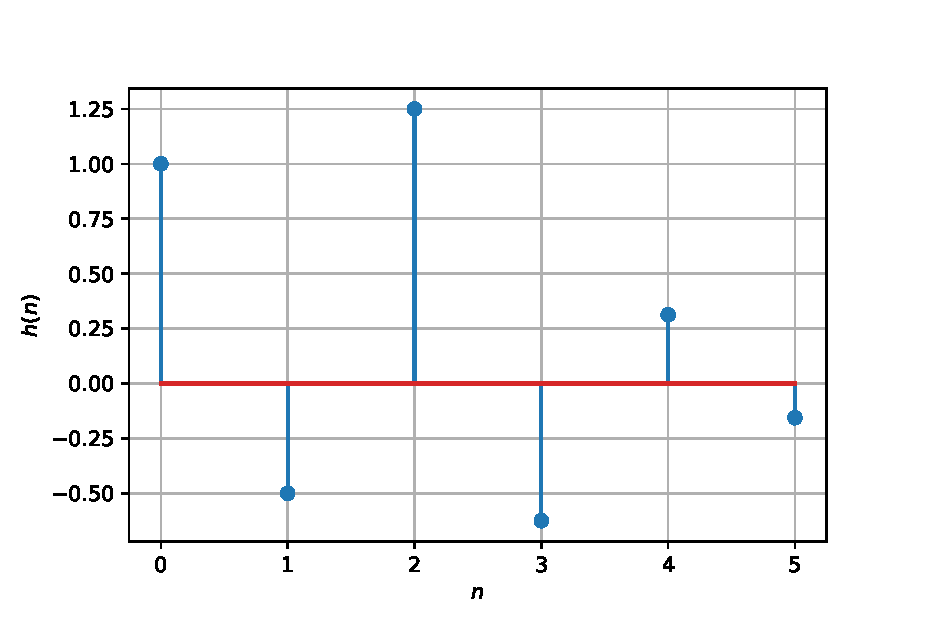
\includegraphics[width=\columnwidth]{./figs/h_n.eps}
    \caption{impulse response : h(n)}
    \label{hn}
\end{figure}

\item FFT of the input signal x(n) is 
\begin{align}
    X(k) = \sum_{n=0}^{N-1} x(n) e^{-j 2 \pi k n / N}, \quad k=0,1 \ldots N-1
\end{align}
\begin{figure}[h!]
    \centering
    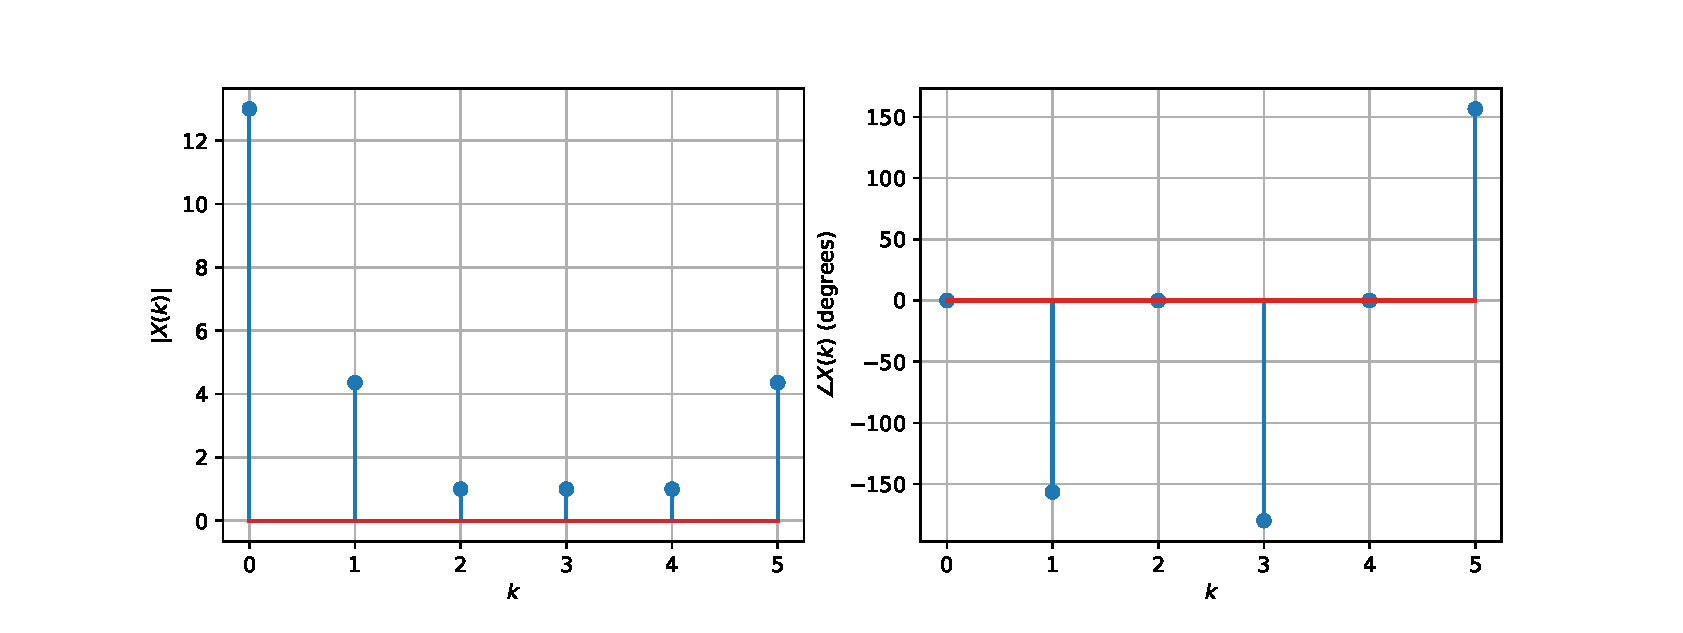
\includegraphics[width=\columnwidth]{./figs/X.eps}
    \caption{FFT of x(n) : X(k)}
    \label{Xk}
\end{figure}
\item FFT of the impulse response h(n) is 
\begin{align}
    H(k) = \sum_{n=0}^{N-1} h(n) e^{-j 2 \pi k n / N}, \quad k=0,1, \ldots, N-1
\end{align}

\begin{figure}[ht]
    \centering
    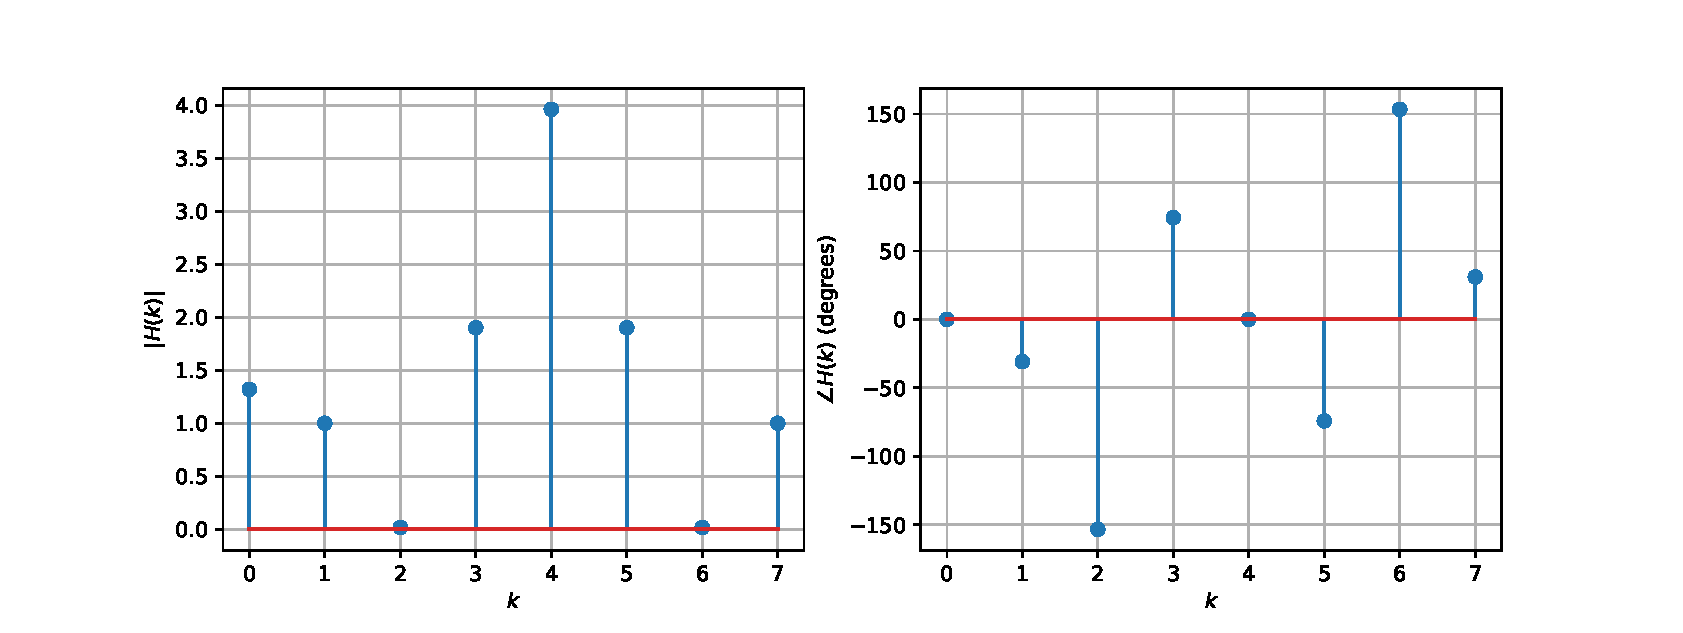
\includegraphics[width=\columnwidth]{./figs/H.eps}
    \caption{FFT of h(n) : H(k)}
    \label{Hk}
\end{figure}

\item  FFT of output Signal y(n) can be computed as 
\begin{align}
    Y(k) = X(k)H(k)
    \label{eq:eq1}
\end{align}

\begin{figure}[ht]
    \centering
    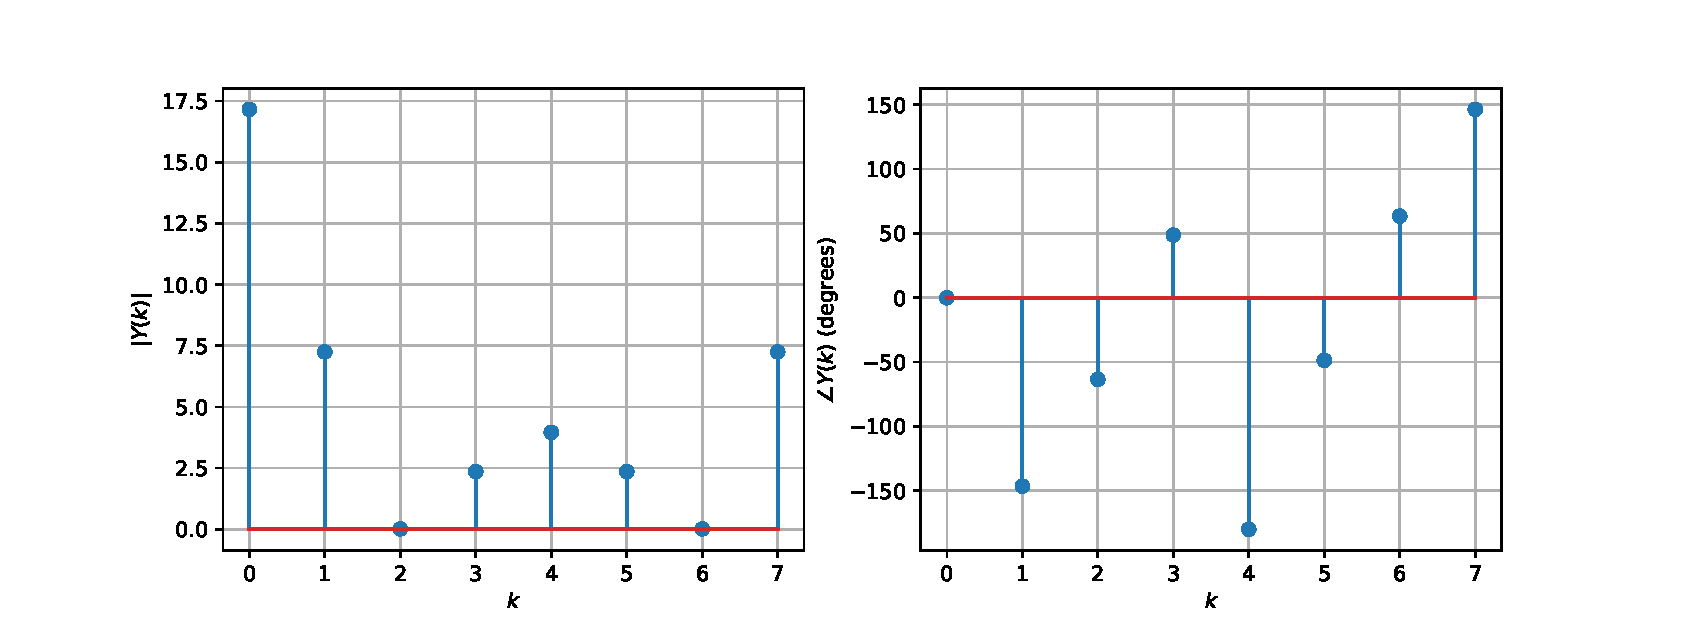
\includegraphics[width=\columnwidth]{./figs/Y.eps}
    \caption{$Y(k) = H(k)X(k)$}
    \label{Yk}
\end{figure}

\item y(n) can be computed by taking IFFT of Y(k)
\begin{align}
    y(n) = \frac{1}{N}\sum_{n=0}^{N-1}Y(k) e^{j 2 \pi n k / N}, \quad k=0,1, \ldots, N-1
\end{align}


\begin{figure}[h!]
    \centering
    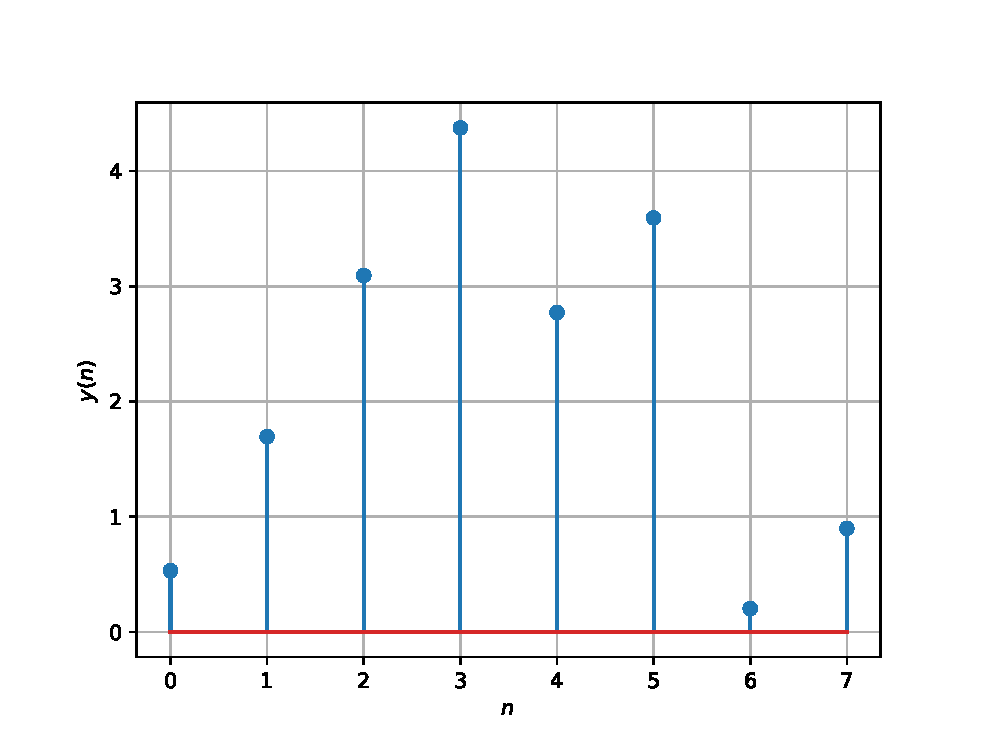
\includegraphics[width=\columnwidth]{./figs/y_n.eps}
    \caption{IFFT of Y(k) : y(n)}
    \label{yn}
\end{figure}
\end{enumerate}

\section{problem}
\begin{enumerate}[label=\thesection.\arabic*.,ref=\thesection.\theenumi]
    \numberwithin{equation}{enumi}
    \item Wherever possible, express all the above equations as matrix equations.
\end{enumerate}
\section{Solution}
\begin{enumerate}[label=\thesection.\arabic*.,ref=\thesection.\theenumi]
    \numberwithin{equation}{enumi}
    \item FFT of signal X(n) 
    \begin{align}
        X(k) \triangleq W_{N}^{nk} x(n), \quad k=0,1, \ldots, N-1
        \label{eq:eq2}
    \end{align}
     where $W_{N}^{n k}=e^{-j 2 \pi k n / N}$ which can be $\mathrm{ex}-$ pressed as:
\begin{align}
\begin{bmatrix} X(0) \\ X(1) \\ X(2) \\ X(3) \\ X(4) \\ X(5) \end{bmatrix}
=
\begin{bmatrix}
1 & 1 & 1 & 1 & 1 & 1 \\ 1 & W_N^1& W_N^2& W_N^3 & W_N^4 & W_N^5\\1 & W_N^2 & W_N^4 & W_N^6 & W_N^8 & W_N^{10}\\1 & W_N^3 & W_N^6 & W_N^9 & W_N^{12} & W_N^{15}\\1 & W_N^4 & W_N^8 & W_N^{12} & W_N^{16} & W_N^{20}\\1 & W_N^5 & W_N^{10} & W_N^{15} & W_N^{20} &W_N^{25}
\end{bmatrix}%
\begin{bmatrix}
x(0) \\ x(1) \\ x(2) \\ x(3) \\ x(4) \\x(5)
\end{bmatrix}
\end{align}

\begin{align}
    \implies \begin{bmatrix} X(0) \\ X(1) \\ X(2) \\ X(3) \\ X(4) \\ X(5) \end{bmatrix}
         =
\begin{bmatrix}
1 +2+3+4+2+1 \\ 1+ (2)e^{-j\pi /3} + ... + (1)e^{-j5\pi /3}\\ 1 + (2)e^{-2j\pi /3} + ... +(1)(e^{-2j5\pi /3}\\ 1 + (2)e^{-3j\pi /3} + ... + (1)e^{-3j5\pi /3}\\ 1 + (2)e^{-4j\pi /3} + ... + (1)e^{-4j5\pi /3}\\ 1 + (2)e^{-5j\pi /3} + ... + (1)e^{-5j5\pi /3}
\end{bmatrix}
\end{align}
On solving,\\

\begin{align}
    \implies \begin{bmatrix} X(0) \\ X(1) \\ X(2) \\ X(3) \\ X(4) \\ X(5) \end{bmatrix}
         =
\begin{bmatrix}
13 + 0j \\ -4 - 1.732j \\ 1 + 0j \\ -1 + 0j \\ 1 + 0j \\ -4 + 1.732j
\end{bmatrix}
\end{align}

\item
Similarly,

\begin{align}
    \begin{bmatrix} H(0) \\ H(1) \\ H(2) \\ H(3) \\ H(4) \\ H(5) \end{bmatrix}
=
\begin{bmatrix}
h(0) + h(1) + h(2) + h(3) + h(4) + h(5) \\h(0) + h(1)e^{-j\pi /3} + ... + h(5)e^{-j5\pi /3}\\h(0) + h(1)e^{-2j\pi /3} + ... + h(5)e^{-2j5\pi /3}\\h(0) + h(1)e^{-3j\pi /3} + ... + h(5)e^{-3j5\pi /3}\\
h(0) + h(1)e^{-4j\pi /3} + ... + h(5)e^{-4j5\pi /3}\\h(0) + h(1)e^{-5j\pi /3} + ... + h(5)e^{-5j5\pi /3}
\end{bmatrix}
\end{align}

On solving,

\begin{align}
\implies
\begin{bmatrix} H(0) \\ H(1) \\ H(2) \\ H(3) \\ H(4) \\ H(5) \end{bmatrix}
=
\begin{bmatrix}
1.28125 + 0j,\\
0.51625 - 0.5141875j,\\
-0.078125 + 1.1095625j,\\
 3.84375 + 0j,\\
-0.071825 - 1.1095625j.\\
 0.515625 + 0.5141875j
\end{bmatrix}
\end{align}

\item Compute $Y(k)$ using 	Eq \eqref{eq:eq1}
\begin{equation}
\renewcommand{\arraystretch}{1.45}
\setlength\arraycolsep{0.01pt}
\begin{bmatrix} 
Y(0) \\ Y(1) \\ Y(2) \\ Y(3) \\ Y(4) \\ Y(5) 
\end{bmatrix}
=
\begin{bmatrix}
X(0)\cdot H(0) \\ X(1)\cdot H(1) \\ X(2)\cdot H(2) \\ X(3)\cdot H(3) \\ X(4)\cdot H(4) \\ X(5)\cdot H(5)
\end{bmatrix}
\end{equation}

Solving,
\begin{equation}
\renewcommand{\arraystretch}{1.45}
\setlength\arraycolsep{0.01pt}
\begin{bmatrix} 
Y(0) \\ Y(1) \\ Y(2) \\ Y(3) \\ Y(4) \\ Y(5) 
\end{bmatrix}
=
\begin{bmatrix}
16.6562+0j \\ -2.95312+1.16372j \\ -0.07812+1.10959j \\ -3.84375-9.27556j \\ -0.07812-1.10959j \\ -2.95312-1.16372j 
\end{bmatrix}
\end{equation}

\item
\begin{align}
    y(n) \triangleq (W_{N}^{nk})^{*} Y(k), \quad n=0,1, \ldots, N-1
\end{align}
where $(W_{N}^{nk})^{*}$ is conjugate of $W_{N}^{nk}$ from \eqref{eq:eq2}.

\begin{align}
    \begin{bmatrix} 
y(0) \\ y(1) \\ y(2) \\ y(3) \\ y(4) \\ y(5) 
\end{bmatrix}
=
\begin{bmatrix}
1.125     +0j \\ 2.28125071+0j \\ 2.6250019 -1.11022302 \times 10^{-16}j \\ 4.37499667-1.47104551\times 10^{-15}j \\ 2.6562481 +6.10622664 \times 10^{-16}j \\ 3.59375262-1.60982339 \times 10^{-15}j 
\end{bmatrix}
\end{align}

\item
Properties :
\begin{enumerate}
    \item symmetry property : \[ W^{k+N/2}_{N} = - W^{k}_{N} \] 
    \item Periodicity property :  \[ W^{k+N}_{N} =  W^{k}_{N} \] 
    \item \[ W^{2}_{N} =  W_{N/2} \] 
\end{enumerate}
\item 
Using properties to derive FFT from DFT :
    \begin{align}
       \mathcal X(k) &=  \sum_{n=0}^{N-1} x(n)W^{kn}_{N}, \quad k=0,1, \ldots, N-1 \\
       &= \sum_{n=even} x(n)W^{kn}_{N} + \sum_{n=odd} x(n)W^{kn}_{N} \\
       &= \sum_{m=0}^{2} x(2m)W^{2mk}_{N} + \sum_{m=0}^{2} x(2m+1)W^{(2m+1)k}_{N} 
    \end{align}
using property c, we get,
    \begin{align}
        \mathcal X(k) &= \sum_{m=0}^{2} x(2m)W^{mk}_{N/2} + W^{k}_{N} \sum_{m=0}^{2} x(2m+1)W^{mk}_{N/2} \\
        &= X_{1}(k) + W^{k}_{N}X_{2}(k)
    \end{align}

\item
\begin{itemize}
    \item X\textsubscript{1}(k) and X\textsubscript{2}(k) are 3 point DFTs of x(2m) and x(2m+1) , m=0,1,2.
    \item X\textsubscript{1}(k) and X\textsubscript{2}(k) are periodic, Hence X\textsubscript{1}(k+3) = X\textsubscript{1}(k) and X\textsubscript{2}(k+3) = X\textsubscript{1}(k).
    \item From performing this step once we can see that number of computations have been reduced\\
    from $N^2$ to $\frac{N^2}{2}$.
\end{itemize}

\item Using the above properties recursively we have implemented radix-2 the Fast-Fourier transform algorithm.

\begin{center}
 \begin{tabular}{||c c c||} 
 \hline
 Algorithm & t$(N=128)$ & t$(N=2048)$ \\ [0.5ex] 
 \hline\hline
 DTFT & 33.2 ms & 7.36 s \\ 
 \hline
 FFT & 1.54 ms & 27.6 ms \\ [1ex] 
 \hline
\end{tabular}
\end{center}

\begin{itemize}
    \item $t(N)$ corresponds to average time of execution for sample size of $N$.
    \item We can observe that as we increase $N$, the difference in execution times is drastically increasing.
    \item From our implementation of radix-2 FFT we can see that complexity is reduced from 
    \\ $\mathcal{O}(n^2)$ to $\mathcal{O}(n\log{}n)$ 
\end{itemize}


\end{enumerate}
\end{document}

